\section{Proposed Method}
\label{sec:methods}

\subsection{Problem Formulation}

We formulate cross-language scene text replacement in video as a structured video-to-video transformation task.

Given an input video:
\[
V = \{F_1, F_2, \dots, F_N\}, \quad F_t \in \mathbb{R}^{H \times W \times 3},
\]
the goal is to produce an output sequence:
\[
V' = \{F'_1, F'_2, \dots, F'_N\},
\]
where all scene text is translated into a target language while preserving geometric consistency, temporal coherence, and photorealistic appearance.

We model each text instance as a track:
\[
T_i = \{Q_i^t, s_i, s'_i\}_{t=1}^N,
\]
where $Q_i^t$ denotes the quadrilateral region at frame $t$, and $s_i, s'_i$ are the source and translated text.

\subsection{Method Overview}

Our key design choice is to decouple text generation from temporal propagation. Instead of editing text independently in each frame, we edit a single high-quality reference frame, and propagate the result across time using explicit geometric and photometric modeling.

This avoids temporal flickering and enables controlled adaptation to viewpoint and appearance changes.

The pipeline consists of five stages:
\begin{itemize}
    \item \textbf{S1: Detection, Tracking, and Reference Selection}
    \item \textbf{S2: Frontalization}
    \item \textbf{S3: Text Editing}
    \item \textbf{S4: Propagation (Lighting + Blur)}
    \item \textbf{S5: Compositing}
\end{itemize}

\begin{center}
    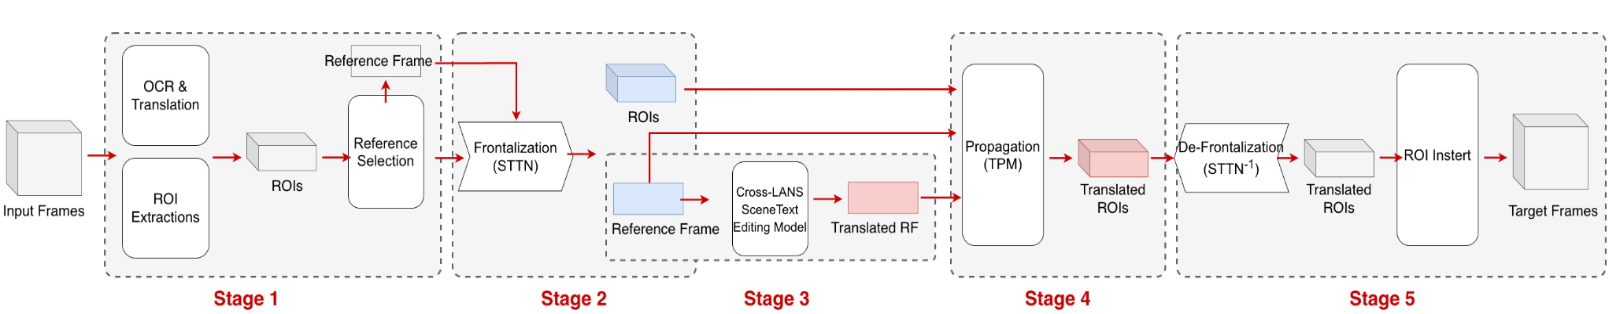
\includegraphics[width=\linewidth]{figures/PipelineDiagram.png}
\end{center}

\noindent\textbf{Figure 1:} Overview of the proposed pipeline. The system consists of five stages: detection and tracking, frontalization, text editing, temporal propagation, and final compositing.

\subsection{S1: Detection, Tracking, and Reference Selection}

This stage produces temporally consistent text tracks from video frames, together with reference frames and dense geometric trajectories for downstream processing.

\subsubsection{Text detection}

We apply PP-OCRv4 on uniformly sampled frames with stride $N$, reducing computational cost while preserving temporal coverage. The detector outputs text quadrilaterals and confidence scores. We filter low-quality detections using OCR confidence thresholding and lexical plausibility constraints based on word frequency statistics, suppressing spurious detections from background textures.

\subsubsection{Track formation}

Detections are associated across frames using a greedy matching strategy that combines geometric and semantic cues. For a detection $d_i^t$ and a candidate match $d_j^{t-1}$, we compute:
\[
S_{\text{match}} = \lambda_1 \, \text{IoU} + \lambda_2 \, \text{sim}_{\text{text}} + \lambda_3 \, \text{sim}_{\text{temp}} + \lambda_4 \, \text{sim}_{\text{dist}},
\]
where IoU measures spatial overlap, text similarity captures lexical consistency, and the remaining terms encode temporal and spatial coherence. A new track is initialized when no match exceeds the acceptance threshold.

\subsubsection{Reference selection}

For each track, we select a reference frame that maximizes visual quality and geometric suitability. The score is defined as:
\[
S_{\text{ref}} = 0.7 \cdot \text{contrast} + 0.3 \cdot \text{frontality},
\]
where contrast is estimated using Otsu-based separation and frontality measures quadrilateral-to-bounding-box area ratio. Additional constraints on OCR confidence, sharpness, and text-length consistency improve robustness.

\subsubsection{Temporal refinement}

We leverage CoTracker~\cite{cotracker} to propagate quadrilateral corner points across frames. Unlike classical optical flow methods such as Lucas--Kanade and Farneback, this learned tracker models long-range temporal dependencies and is robust to large motion and occlusion. The resulting trajectories are refined using Kalman filtering followed by exponential moving average (EMA) smoothing to reduce jitter while preserving temporal coherence.

Overall, S1 outputs temporally consistent text tracks, each containing per-frame quadrilateral annotations, a selected reference frame, and smoothed dense trajectories.

\subsection{S2: Frontalization}

Given a set of tracked text quadrilaterals, we normalize each instance into a canonical frontal coordinate system using planar homography transformations. For each detection, we estimate a mapping from image space to a canonical rectangle derived from the reference geometry of the track.

In the general case, homographies are computed using either the four quadrilateral corners or a denser set of tracked grid points when available. This enables a more robust least-squares estimation under motion and deformation, improving stability over corner-only alignment.

The canonical space is defined per track based on the geometry of the reference quadrilateral, ensuring consistent scale and aspect ratio across all frames. Each frame-specific transformation is then expressed as:
\[
H_{t \rightarrow c},
\]
which maps image coordinates into this normalized frontal space, effectively removing perspective distortion and enabling pixel-aligned correspondence across time.

When available, a learned refinement module further improves geometric accuracy by predicting residual corrections between reference and target canonical regions. These corrections are integrated into the estimated homography, yielding refined transformations that compensate for residual misalignment.

Overall, S2 produces a set of geometry-normalized text regions in a unified coordinate system, which serves as the foundation for precise text editing in subsequent stages.

\subsection{S3: Text Editing}

This stage performs cross-lingual text replacement on the reference frame within canonical space. Given the frontalized representation from S2, editing is applied once per track at the reference frame and later propagated to other frames.

We employ AnyText2, a diffusion-based scene text editing model built on a Stable Diffusion backbone. The model supports multilingual text replacement while preserving visual attributes such as font style, color, and texture consistency with the surrounding scene.

Since AnyText2 is provided as an external system, we deploy it as a dedicated inference service following the original specifications. The model is executed via a remote server exposing a Gradio-based interface, and our pipeline communicates with it through API calls. This design allows seamless integration while preserving compatibility with the original implementation and avoiding modifications to the underlying model.

\subsubsection{Context-aware adaptive editing}

To improve robustness, we expand the editing region to include surrounding scene context, providing additional cues for illumination and texture consistency. 

To further handle variable-length translations, we introduce an adaptive masking strategy that adjusts the editable region based on the estimated spatial extent of the target text. This prevents over-generation in empty regions and improves alignment for both long-to-short and short-to-long translations.

\subsubsection{Background reconstruction and output}

Occluded background regions introduced by mask adjustments are reconstructed using an auxiliary inpainting model (SRNet), reducing artifacts around edited text regions and ensuring seamless integration into the scene.

The final output of this stage is a geometrically consistent edited region in canonical space:
\[
R_i^{\text{edit}}.
\]

\subsection{S4: Propagation via Appearance Modeling}

We propagate $R^{\text{edit}}_i$ from the reference frame to all remaining frames by modeling two types of appearance variation: illumination changes and motion blur. The stage operates in canonical frontal space and consists of two sequential adaptation modules.

\subsubsection{Lighting Correction Module (LCM)}

We first correct frame-dependent illumination using the Lighting Correction Module (LCM), adapted from STRIVE~\cite{strive}. The module operates on inpainted background regions, obtained using a pretrained background inpainter (e.g., SRNet or Hi-SAM-based inpainting), which removes text content while preserving scene structure.

Given the inpainted reference and target backgrounds, we compute a per-pixel multiplicative correction map:
\[
R^{\text{light}}_t = R^{\text{edit}} \cdot \frac{I_t^p + \epsilon}{I_{\text{ref}}^p + \epsilon},
\]
where $I_t^p$ and $I_{\text{ref}}^p$ denote the inpainted target and reference backgrounds in canonical space. We optionally stabilize this estimate using neighboring frames and temporal exponential moving average (EMA), improving robustness under noisy inpainting artifacts.

This step produces a lighting-aligned intermediate representation $R^{\text{light}}_t$.

\subsubsection{Blur Modeling via BPN}

To handle motion blur variations across frames, we introduce a Blur Prediction Network (BPN), trained to estimate per-frame blur parameters conditioned on reference-target canonical pairs.

The model is trained in two stages: (i) supervised learning on synthetically blurred data with known kernel parameters, and (ii) self-supervised refinement on real video sequences.

At inference time, BPN predicts spatial blur parameters $(\sigma_x, \sigma_y, \rho, w)$ for each target frame. A differentiable Gaussian blur operator is then applied:
\[
R^{\text{blur}}_t = \text{BPN}(R^{\text{light}}_t),
\]
ensuring that the final rendered text matches the motion characteristics of each frame.

\subsubsection{Propagation Pipeline}

The full propagation process can be summarized as:
\[
R^{\text{edit}} \rightarrow \text{LCM} \rightarrow \text{BPN} \rightarrow R_t,
\]
where each stage progressively adapts appearance while preserving geometric consistency from S2.

Overall, S4 produces a temporally coherent set of edited ROIs that are consistent in both illumination and motion blur across the video sequence.

\subsection{S5: Compositing}

Each propagated region is mapped back to the original frame using the inverse homography:
\[
H_{c \rightarrow t}.
\]

To ensure spatial accuracy and computational efficiency, we perform localized warping within the target bounding region instead of processing the full frame. The warped region is then blended into the frame using alpha compositing with a feathered mask, which ensures smooth boundary transitions and reduces visible edge artifacts.

This produces the final output frames $\{F'_t\}$.

\subsection{Methodology Conclusions}

Our method combines explicit geometric normalization with learned appearance adaptation. Notably:
\begin{itemize}
    \item Frontalization enables consistent editing and alignment.
    \item LCM provides deterministic illumination transfer.
    \item BPN models dynamic blur not captured by classical methods.
\end{itemize}

This decomposition allows high-quality, temporally consistent text replacement without requiring per-frame generative inference.